\documentclass[tikz,border=3mm]{standalone}
\usetikzlibrary{decorations.pathreplacing} % For curve labeling

\begin{document}
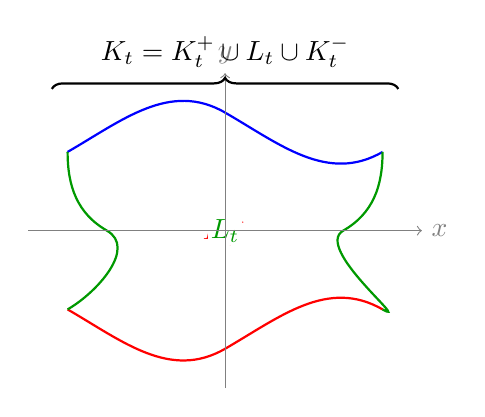
\begin{tikzpicture}[
    curve/.style={thick, smooth, tension=0.7},
    label/.style={midway, fill=white, inner sep=1pt}
]
    % Draw K_t^+ (upper curve)
    \draw[curve, color=blue] 
        ( -2, 1) to[out=30, in=150] ( 0, 1.5) 
                 to[out=330, in=210] ( 2, 1)
        node[label] {$K_t^+$};
    
    % Draw K_t^- (lower curve)
    \draw[curve, color=red] 
        ( -2,-1) to[out=330, in=210] ( 0,-1.5) 
                 to[out=30, in=150] ( 2,-1)
        node[label] {$K_t^-$};
    
    % Draw L_t (connecting curve)
    \draw[curve, color=green!60!black] 
        ( 2, 1) to[out=270, in=30] (1.5, 0)
                to[out=210, in=330] (2,-1)
        node[label] {$L_t$};
    \draw[curve, color=green!60!black] 
        (-2, 1) to[out=270, in=150] (-1.5, 0)
                to[out=330, in=30] (-2,-1);
    
    % Axes for reference (optional)
    \draw[->, thin, gray] (-2.5,0) -- (2.5,0) node[right] {$x$};
    \draw[->, thin, gray] (0,-2) -- (0,2) node[above] {$y$};
    
    % Union indicator (bracket)
    \draw[decorate, decoration={brace, amplitude=4pt}, thick]
        (-2.2,1.8) -- (2.2,1.8) node[midway, above=4pt] {$K_t = K_t^+ \cup L_t \cup K_t^-$};
\end{tikzpicture}
\end{document}